% ============================================================================
% APPENDIX — Journal of Big Data
% ============================================================================

\section{Evaluation Details}
\label{app:decoding}

\subsection{Models}
We evaluate three frontier-class LLMs:
\begin{itemize}[nosep]
\item \textbf{Gemini~2.5~Flash} (Google, closed-weight, accessed via the
Generative Language API). A multimodal model optimized for speed and
accuracy at scale.
\item \textbf{DeepSeek-V3} (DeepSeek, 671B parameter Mixture-of-Experts,
MIT licensed, accessed via API). An open-weight model competitive with
closed-source alternatives.
\item \textbf{Qwen2.5-72B} (Qwen Team, 72B dense model,
Apache-2.0, accessed via API). An open-weight model with strong
reasoning capabilities.
\end{itemize}
All three models use greedy decoding ($\tau{=}0$, $p{=}1.0$) with a single
deterministic pass per question for exact reproducibility. No few-shot
examples or chain-of-thought prompting is used.

\subsection{Scoring Methodology}
\textbf{Exact Match (EM)} is the primary metric. The predicted answer must
exactly match the gold answer after the following canonicalization steps:
\begin{enumerate}[nosep]
\item \textit{List canonicalization}: lists are lowercased and sorted
alphabetically; order does not matter.
\item \textit{Path validation}: for \texttt{join\_path} questions,
alternative shortest paths of equal length are validated against the FK
adjacency matrix to accept valid alternatives.
\item \textit{Boolean normalization}: ``yes''/``true''/``1'' are equivalent;
``no''/``false''/``0'' are equivalent.
\item \textit{Whitespace and case}: all comparisons are
case-insensitive after stripping whitespace.
\end{enumerate}
\textbf{F1} is computed as token-level overlap between predicted and gold
answer sets, used as a secondary metric for partial credit.

\subsection{Baseline Implementation Details}
\textbf{Vector-RAG} uses \texttt{all-MiniLM-L6-v2}~\cite{reimers2019sentencebert}
embeddings (384 dimensions) with FAISS exact search ($k{=}15$ retrieved
chunks per question). Schema elements (tables, columns, FK edges, lineage
edges) are embedded as natural language descriptions.

\textbf{Graph-Augmented} computes 3-hop BFS neighborhoods from mentioned
table names using NetworkX. The subgraph is serialized as structured text
(node list + edge list with types).

\textbf{Tool-Use} provides 9 graph algorithm tools:
\texttt{shortest\_path}, \texttt{connected\_components},
\texttt{check\_fk\_adjacency}, \texttt{get\_lineage\_forward},
\texttt{get\_lineage\_reverse}, \texttt{transitive\_lineage},
\texttt{get\_component\_of}, \texttt{get\_fk\_neighbors},
\texttt{list\_tables}. The LLM receives tool definitions and a schema
summary, then generates up to 3 tool calls per question in a multi-turn
conversation.

\textbf{ReAct-Code} provides a Python REPL with NetworkX pre-loaded.
The LLM writes and executes Python code to query the schema graph
directly, with up to 5 code execution rounds per question. This tests
whether the LLM can translate graph-reasoning tasks into correct
algorithmic implementations.

\subsection{Statistical Treatment}
All figures include 95\% bootstrap confidence intervals computed via
2,000 resamples over questions. Per-question results (JSON files) are
released for community bootstrap and stratification analyses. Greedy
decoding ensures deterministic reproducibility without requiring
multiple runs or confidence intervals over random seeds.

\FloatBarrier
\section{Tier~2 Extended Results (Qwen2.5-72B)}
\label{app:tier2}

Qwen2.5-72B on Tier~2 (Syn-Logistics, \{=}433\$) shows the same
tools-essential-yet-insufficient pattern as Gemini and DeepSeek:
\texttt{cascade\_count} reaches near 100\% with Tool-Use vs.\ 0\% without;
on compositional subtypes (\texttt{multi\_hop\_trace}, \texttt{shared\_source})
Qwen plateaus at 25--30\%, confirming cross-model generality of the ceiling.
Full results are available in the released per-question JSON files.

\FloatBarrier
\section{Hop-Distance Analysis}
\label{app:hop-distance}

\begin{figure}[h!]
\centering
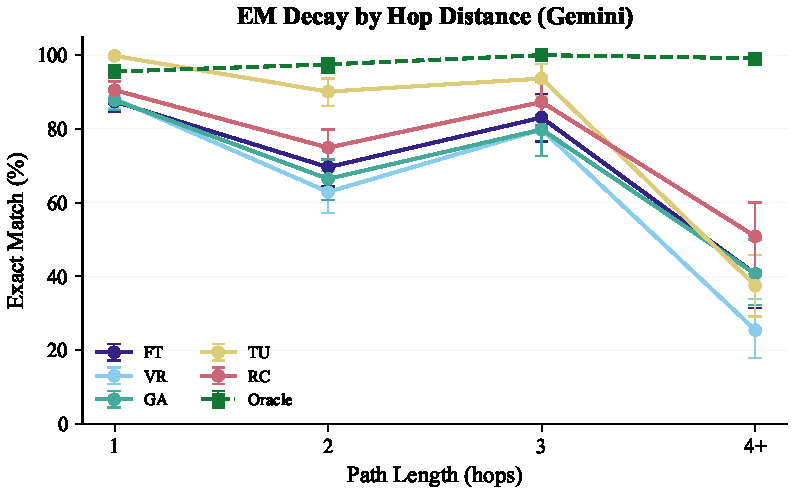
\includegraphics[width=0.85\linewidth]{figures/hop_distance_decay.pdf}
\caption{EM by gold path length (Gemini, representative). Static baselines collapse beyond
3~hops while Tool-Use degrades more gracefully, confirming that interactive
graph access is essential for multi-hop reasoning. DeepSeek and Qwen
show the same qualitative pattern.}
\label{fig:hop_decay_app}
\end{figure}

\begin{table}[h!]
\centering
\caption{Minimum evidence hops per subtype (Syn-Logistics). 45.4\% of
questions exceed the GA 3-hop BFS radius, explaining the performance gap
between static and agentic baselines.}
\label{tab:hop-distance}
\small
\begin{tabular}{lrrrc}
\toprule
Subtype & $n$ & Exceeds 3h & \% & GA EM \\
\midrule
count            & 26 & 26 & 100\% & 100\% \\
membership       & 20 & 20 & 100\% & 0\% \\
combined\_impact & 34 & 34 & 100\% & 0\% \\
full\_enum       & 25 & 25 & 100\% & 100\% \\
connected        & 25 & 25 & 100\% & 100\% \\
isolation        & 25 & 25 & 100\% & 100\% \\
transitive       & 29 &  4 &  14\% & 93\% \\
hop\_count       & 44 &  5 &  11\% & 100\% \\
direct\_fk       & 36 &  3 &   8\% & 100\% \\
join\_path       & 26 &  2 &   8\% & 81\% \\
multi\_source    & 42 &  0 &   0\% & 95\% \\
forward          & 20 &  0 &   0\% & 100\% \\
reverse          & 20 &  0 &   0\% & 100\% \\
\midrule
\textbf{Total}   & 372 & 169 & \textbf{45.4\%} & 83.1\% \\
\bottomrule
\end{tabular}
\end{table}

\FloatBarrier
\section{Dataset Construction Details}
\label{app:datasets}

\subsection{Syn-Logistics Design}
The Syn-Logistics dataset was constructed to guarantee $n\geq20$ for every
subtype by building three parallel 4-hop lineage chains across five
connected components. Table names are drawn from a Domain Dictionary of
realistic supply-chain terminology to prevent semantic collapse under
obfuscation. The schema contains 64 tables, 96 FK edges, 35 lineage edges,
and 372~Tier~1 + 433~Tier~2 questions.

\subsection{Lineage Edge Curation}
Lineage (derived\_from) edges are curated per dataset:
\begin{itemize}[nosep]
\item \textbf{AdventureWorks}: Extracted from official Microsoft reference
documentation mapping OLTP source tables to DW dimension/fact tables (39~edges).
\item \textbf{TPC-DS}: No lineage edges; schema is a pure star/snowflake FK graph.
\item \textbf{TPC-DI}: Derived from the official TPC-DI specification
defining staging$\to$dimension$\to$fact transformation flows (21~edges).
\item \textbf{OMOP CDM}: Derived from OHDSI ETL convention guides mapping
source vocabularies and clinical tables to standardized CDM tables (21~edges).
\item \textbf{Syn-Logistics}: Defined by construction: three parallel
4-hop chains (raw$\to$staging$\to$dimension$\to$mart) per connected
component (35~edges). All lineage edges are validated by verifying that
the source table's schema semantically feeds the target table's schema.
\end{itemize}

\section{Example Questions and Predictions}
\label{app:examples}

\FloatBarrier
\begin{table}[h!]
\centering
\caption{Representative questions across difficulty levels and categories,
with gold answers and Tool-Use (TU) predictions.
\cmark~=~correct, \xmark~=~incorrect. Tool-Use succeeds on lookup-style
questions but fails on exhaustive enumeration and multi-hop composition.}
\label{tab:examples}
\scriptsize
\begin{tabular}{p{0.12\linewidth}p{0.35\linewidth}p{0.22\linewidth}p{0.22\linewidth}}
\toprule
\textbf{Subtype} & \textbf{Question} & \textbf{Gold} & \textbf{TU Pred.} \\
\midrule
\texttt{direct\_fk} \newline \textit{Easy} &
Is there a direct FK between \texttt{DW.DimProduct} and
\texttt{DW.Fact\-Internet\-Sales}? &
yes &
yes \cmark \\
\midrule
\texttt{join\_path} \newline \textit{Medium} &
What is the shortest FK path from \texttt{DW.Dim\-Customer} to
\texttt{DW.Dim\-Product}? &
{[}DimCustomer, Fact\-Internet\-Sales, DimProduct{]} &
{[}DimCustomer, Fact\-Internet\-Sales, DimProduct{]} \cmark \\
\midrule
\texttt{membership} \newline \textit{Hard} &
Which connected component contains \texttt{DW.DimCurrency}? List all
tables in that component. &
{[}DimCurrency, Fact\-Currency\-Rate, DimDate, ...{]} (12~tables) &
{[}DimCurrency{]} \xmark \\
\midrule
\texttt{combined\_impact} \newline \textit{Hard} &
Which tables are transitively affected (via lineage and FK) if
\texttt{raw\_purchase\_orders} is modified? &
{[}stg\_purchase\_orders, dim\_supplier, ...{]} (8~tables) &
{[}stg\_purchase\_orders{]} \xmark \\
\midrule
\texttt{cascade\_count} \newline \textit{Tier~2} &
How many downstream rows would be affected if we delete \texttt{shipment\_id=SH042}
from \texttt{raw\_shipments}? &
147 &
147 \cmark \\
\midrule
\texttt{multi\_hop\_trace} \newline \textit{Tier~2} &
Trace the full provenance chain of \texttt{order\_id=ORD-2891} in
\texttt{mart\_profit\_analysis}. &
{[}raw\_purchase\_orders $\to$ stg\_orders $\to$ dim\_product $\to$
mart\_profit\_analysis{]} &
{[}raw\_purchase\_orders, mart\_profit\_analysis{]} \xmark \\
\bottomrule
\end{tabular}
\end{table}

\section{Reproducibility Statement}
\label{app:reproducibility}

All code, data, and evaluation scripts are publicly available at
\url{https://github.com/AJamal27891/dw-bench}. The benchmark datasets
(including schema graphs, QA pairs, and value-level data) will be released
on HuggingFace at \url{https://huggingface.co/datasets/AJamal27891/dw-bench}.
Per-question result JSON files enable exact reproduction of all reported
numbers. Greedy decoding ($\tau{=}0$) ensures deterministic outputs.
